%%
% La siguiente plantilla esta basada en el siguiente enlace:
% http://academic.reed.edu/physics/courses/Physics332.s08/reports.html
% La plantilla original puede descargarse de ese sitio
% Se dejo parte del texto original en inglés para ilustar el uso de la plantilla
% Se hicieron algunas modificaciones para ajustar el idioma y otros detalles para 
% completar un reporte técnico breve pero muy puntual
% Modificación Inicial: Marco Aurelio Nuno Maganda - 11/SEP/2014
% 
% Enlace a la documentación del tipo de documento base (revtex4)
% http://mirror.hmc.edu/ctan/macros/latex/contrib/revtex/doc/latex/revtex/source/revtex4-1.pdf
%
% En algunas distribuciones es necesario instalar el paquete texlive-publishers
%
%\documentclass[letterpaper,aps,twocolumn,pre,nofootinbib]{revtex4}
%\documentclass[twocolumn]{article}
\documentclass[conference]{IEEEtran}

\usepackage[spanish]{babel}
\usepackage{amsmath,amssymb,amsfonts,amsthm}
\usepackage{graphicx}
%\usepackage{bbm}
\usepackage[utf8]{inputenc} % Caracteres en Español (Acentos, ñs)
\usepackage{url} % ACENTOS
\usepackage{hyperref} % Referencias
\usepackage{subfig}
\usepackage{lipsum}
\usepackage{balance}


%%%%%%%%%%%%%%%%%%%%%%%%%%%%%%%%%%%%%%%%%%%%%
% PARCHE PARA ELIMINAR LA FECHA DEL DOCUMENTO
% 
\usepackage{etoolbox}
\makeatletter
% \frontmatter@RRAP@format is responsible for the parentheses
\patchcmd{\frontmatter@RRAP@format}{(}{}{}{}
\patchcmd{\frontmatter@RRAP@format}{)}{}{}{}
%\renewcommand\Dated@name{}
\makeatother	
% FIN DEL PARCHE
% 
%%%%%%%%%%%%%%%%%%%%%%%%%%%%%%%%%%%%%%%%%%%%%

%%%%%%%%%%%%%%%%%%%%%%%%%%%%%%%%%%%%%%%%%%%%%
% PARCHE PARA PERMIRIR UTILIZAR BIBLATEX EN ESTA PANTLLA
%\PassOptionsToPackage{square,numbers}{natbib}
%\RequirePackage{natbib}  
%%%%%%%%%%%%%%%%%%%%%%%%%%%%%%%%%%%%%%%%%%%%%

\usepackage[backend=bibtex,sorting=none]{biblatex}
% Estas lineas permiten romper los hipervinculos muy largos !!!!
\setcounter{biburllcpenalty}{7000}
\setcounter{biburlucpenalty}{8000}
\addbibresource{references.bib}

% Actualiza en automático la fecha de las citas de internet a la fecha de la compilación del documento
\usepackage{datetime}
\newdateformat{specialdate}{\twodigit{\THEDAY}-\twodigit{\THEMONTH}-\THEYEAR}
\date{\specialdate\today}

% la sentencia \burl en las citas... 
\usepackage[hyphenbreaks]{breakurl}

\renewcommand\spanishtablename{Tabla}
\renewcommand\spanishfigurename{Figura}

%\usepackage{datetime}
%\newdateformat{specialdate}{\twodigit{\THEDAY}-\twodigit{\THEMONTH}-\THEYEAR}
%\newdateformat{specialdate}{\twodigit{\THEDAY}-\THEYEAR}
%\date{\specialdate\today}


\begin{document}
%%%%%%%%%%%%%%%%%%%%%%%%%%%%%%%%%%%%%%%%%%%%%
% Definitions
%
%
% Define your special symbols here
%
%%%%%%%%%%%%%%%%%%%%%%%%%%%%%%%%%%%%%%%%%%%%%

% use to set width of figures
\newcommand{\breite}{0.9} %  for twocolumn
\newcommand{\RelacionFiguradoscolumnas}{0.9}
\newcommand{\RelacionFiguradoscolumnasPuntoCinco}{0.45}


%%%%%%%%%%%%%%%%%%%%%%%%%%%%%%%%%%%%%%%%%%%%%
% End Definitions
%%%%%%%%%%%%%%%%%%%%%%%%%%%%%%%%%%%%%%%%%%%%%


%Title of paper
\title{Proyecto en Equipo Unidad 3 \\  Skin Change}

% Trabajo Individual
\author{\IEEEauthorblockN{
Jose Luis Osorio Martinez\\
Maria Guadalupe Saavedra Gonzalez \\
Deisy Dalila De La Fuente Alvarado\\
Aris Uriel Torres Desilos\\
Jesus Roberto Avalos Flores\\ 
\IEEEauthorrefmark{0}}
% En caso de trabajos en equipo, poner a todos los autores en estricto ORDEN ALFABETICO
%\author{\IEEEauthorblockN{Michael Shell\IEEEauthorrefmark{1},
%Homer Simpson\IEEEauthorrefmark{1},
%James Kirk\IEEEauthorrefmark{1}, 
%Montgomery Scott\IEEEauthorrefmark{1} and
%Eldon Tyrell\IEEEauthorrefmark{1}}
\IEEEauthorblockA{\IEEEauthorrefmark{1}Ingeniería en Tecnologías de la Información\\
Universidad Politécnica de Victoria}
}


%\date{}

\maketitle

\begin{abstract} 
Este proyecto describe el desarrollo de SkinChange, una aplicación móvil para Android que utiliza realidad aumentada para modificar el color de la piel en tiempo real. Usando la biblioteca de visión por computadora OpenCV, la aplicación detecta las áreas de piel mediante la combinación de los espacios de color HSV y YCrCb\cite{c1}. Una vez aislada, la piel puede ser aclarada u oscurecida con un control deslizante. La solución permite alternar entre cámaras y capturar fotos con el efecto aplicado, demostrando una aplicación práctica de la manipulación de imágenes en tiempo real.
\end{abstract}

%\maketitle must follow title, authors, abstract, \pacs, and \keywords

\section{Introducción}
La realidad aumentada (RA) ha transformado la manera en que interactuamos con el mundo digital, superponiendo elementos virtuales en el entorno real. Este proyecto se enfoca en una aplicación específica de la RA: la alteración de la luminosidad del color de la piel, permitiendo aclararla u oscurecerla en tiempo real\cite{c2}.
El desarrollo de la aplicación, llamada SkinChange, se basa en los principios de visión por computadora, utilizando la biblioteca OpenCV para Android. La lógica central se inspira en un método de detección de piel que combina los espacios de color HSV y YCrCb para lograr una segmentación precisa. A diferencia de un filtro simple, esta aplicación identifica de forma dinámica las áreas de piel, asegurando que solo esas regiones se vean afectadas por el ajuste de color.
Diseñada para ser intuitiva, la aplicación permite al usuario controlar el efecto con un simple control deslizante y capturar el resultado con solo un toque. Esta combinación de detección de piel, procesamiento en tiempo real y una interfaz de usuario sencilla convierte a SkinChange en una herramienta versátil y un claro ejemplo del potencial de la realidad aumentada en dispositivos móviles\cite{c3}.

\section{Desarrollo Experimental}
El desarrollo de la aplicación móvil SkinChange se realizó a través de un enfoque experimental, centrado en el procesamiento de video en tiempo real para la detección y alteración del tono de la piel. Se implementaron distintas fases, cada una enfocada en un aspecto clave del sistema, desde la captura del video hasta la aplicación del efecto y la interacción con el usuario\cite{c4}.
\subsection{Fase 1: Detección y Segmentación de la Piel}
Esta fase inicial se centró en el desarrollo de un algoritmo robusto para la detección de las áreas de piel dentro del flujo de video.
\begin{itemize}
\item Conversión del espacio de color: Se utilizó la clase JavaCameraView de OpenCV para obtener los fotogramas de la cámara. Cada fotograma RGB se convirtió a los espacios de color HSV (Hue, Saturation, Value) y YCrCb (Luminancia, Crominancia de rojo, Crominancia de azul) para facilitar la detección\cite{c5}.
\item Creación de máscaras binarias: Se aplicaron umbrales de color predefinidos en ambos espacios, usando la función Core.inRange para generar dos máscaras binarias, una para HSV (mMaskHSV) y otra para YCrCb (mMaskYcc), donde los píxeles de la piel se marcan con un valor alto.
\item Combinación de máscaras: Para maximizar la precisión y reducir los falsos positivos (como objetos de color similar a la piel), se combinaron ambas máscaras mediante una operación lógica AND (Core.bitwiseand), resultando en una máscara final que representa de manera precisa las áreas de la piel.
\end{itemize}

\subsection{Fase 2: Aplicación del Efecto y Suavizado}
Esta fase se dedicó a la manipulación del color de la piel detectada y a la integración suave del efecto en el fotograma original.
\begin{itemize}
\item Ajuste de luminosidad: El canal V (Valor) del espacio de color HSV, que controla la luminosidad, se aisló para su manipulación. Un factor de ganancia se aplicó a estos valores de píxel para aclararlos u oscurecerlos, basándose en la posición de un control deslizante en la interfaz de usuario.
\item Suavizado del efecto: Para evitar bordes ásperos y transiciones abruptas en el efecto, se aplicó un desenfoque Gaussiano (Imgproc.GaussianBlur)\cite{c6} a la máscara de piel final. Esto creó una máscara "emplumada" que permite una mezcla gradual y natural entre las áreas modificadas y las no modificadas del fotograma\cite{c7}.
\item Mezcla de fotogramas: Se utilizó la máscara suavizada para mezclar el fotograma original con el fotograma modificado. Esto aseguró que solo las áreas de la piel tuvieran el efecto aplicado, mientras que el resto de la imagen permaneció inalterado.
\end{itemize}

\subsection{Fase 3: Interfaz de Usuario y Funcionalidades Adicionales}
Esta fase abarcó el desarrollo de los elementos interactivos que permiten al usuario controlar la aplicación y utilizar sus funciones complementarias.
\begin{itemize}
\item Control de filtros y luminosidad: Se implementó un control deslizante (SeekBar) para ajustar la intensidad del efecto, con un TextView asociado para mostrar el valor actual. Un Switch permite al usuario activar o desactivar el filtro de la piel\cite{c8}.
\item Alternar cámaras y captura de imagen: Se añadieron botones para alternar entre la cámara frontal y trasera (btnSwitchCam). Adicionalmente, se incluyó una funcionalidad de captura de imagen (btnCapture)\cite{c9} que convierte el fotograma procesado en un archivo de imagen y lo guarda en la galería del dispositivo.
\item Manejo de permisos: La aplicación gestiona automáticamente los permisos de la cámara y de almacenamiento (Manifest.permission.CAMERA y Manifest.permission.WRITEEXTERNALSTORAGE) para garantizar un funcionamiento correcto y la capacidad de guardar imágenes.
\end{itemize}

\section{Resultados}
El desarrollo del proyecto SkinChange ha culminado en una aplicación funcional que valida los objetivos establecidos en la fase de introducción. Los resultados obtenidos demuestran la viabilidad de la manipulación de imágenes en tiempo real a través de la realidad aumentada en un entorno móvil.

Se logró implementar con éxito un algoritmo de detección de piel robusto, combinando los espacios de color HSV y YCrCb. Las pruebas en tiempo real mostraron que el método es efectivo para identificar las áreas de piel en los fotogramas de la cámara, incluso bajo diferentes condiciones de iluminación. Esto permitió generar una máscara binaria precisa que sirve como base para la aplicación del efecto.

\begin{figure}[htbp]
\centering
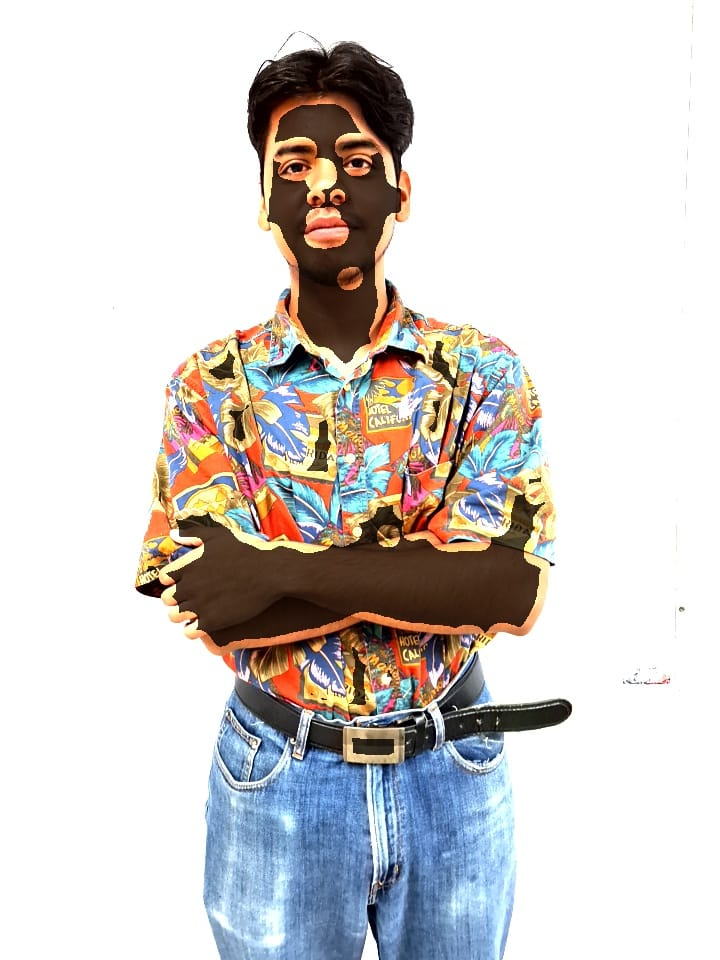
\includegraphics[width=0.45\textwidth]{Imagenes/ejemplo_mascara_piel.jpg}
\caption{Captura de pantalla mostrando la detección de la piel con la máscara generada.}
\label{fig:mascara_piel}
\end{figure}

\begin{figure}[htbp]
\centering
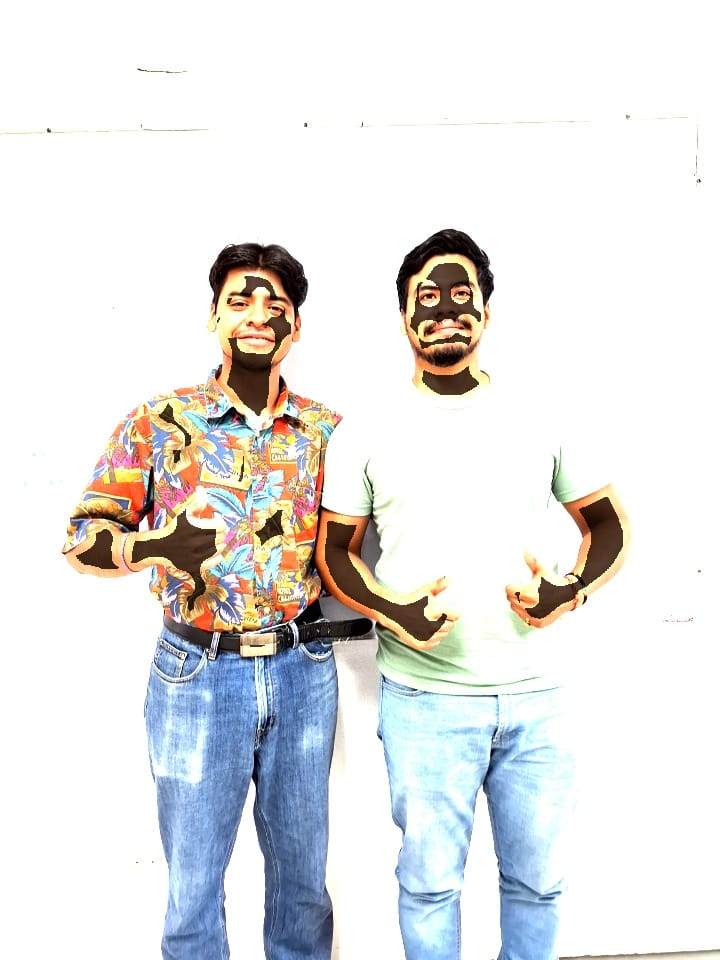
\includegraphics[width=0.45\textwidth]{Imagenes/dos_sujetos.jpg}
\caption{Captura de pantalla mostrando la detección de la piel en dos sujetos de prueba.}
\label{fig:mascara_piel}
\end{figure}

La funcionalidad principal de la aplicación, el ajuste de la luminosidad de la piel, operó en tiempo real. El control deslizante (SeekBar) permitió a los usuarios aclarar u oscurecer la piel dinámicamente. El uso de un desenfoque Gaussiano en la máscara aseguró una mezcla ligeramente natural y transiciones suaves entre las áreas modificadas y las no modificadas, evitando los bordes ásperos y mejorando la calidad visual del efecto.

\begin{figure}[htbp]
\centering
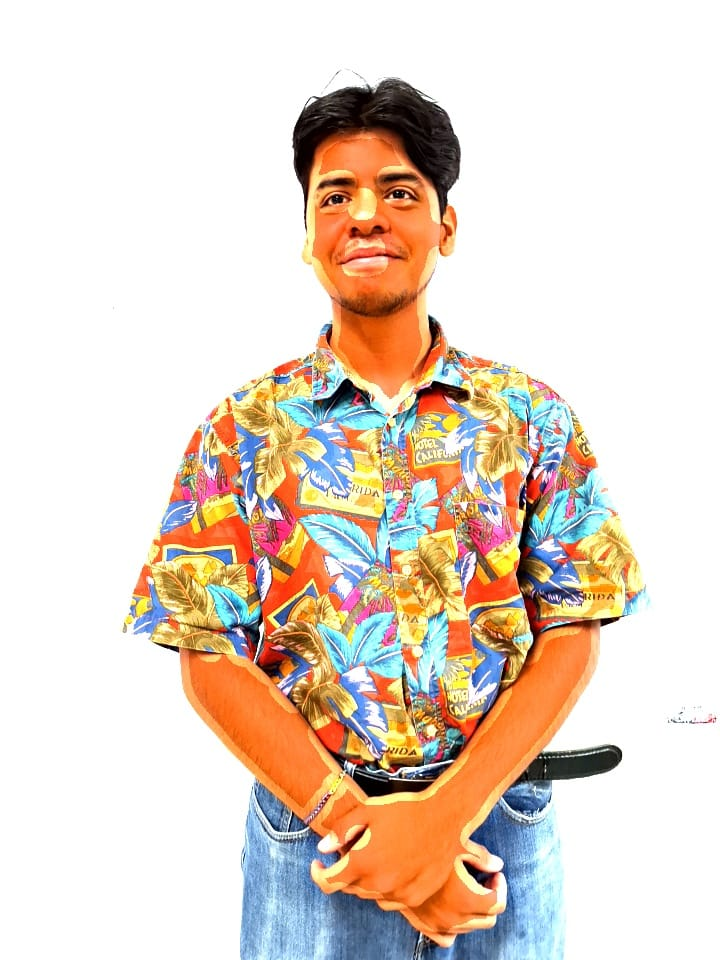
\includegraphics[width=0.45\textwidth]{Imagenes/ejemplo_efecto_aplicado.jpg}
\caption{Aplicación del efecto de luminosidad en la piel en tiempo real.}
\label{fig:efecto_luminosidad}
\end{figure}

Las funcionalidades complementarias de la aplicación, esenciales para la experiencia del usuario, se implementaron correctamente:
\begin{itemize}
\item Alternancia de cámaras: El botón para alternar cámaras funcionó de manera eficiente, permitiendo al usuario cambiar entre la cámara frontal y trasera sin interrupciones.
\item Captura de imagen: La función de captura (btnCapture) guardó con éxito los fotogramas procesados en la galería del dispositivo.
\item Control de filtros: La opción de activar o desactivar el filtro de la piel (Switch) brindó control total sobre la aplicación del efecto.
\end{itemize}

Los resultados finales demuestran que SkinChange es una aplicación de realidad aumentada plenamente operativa. El proyecto valida la viabilidad de usar la biblioteca OpenCV en dispositivos móviles para el procesamiento de video en tiempo real. La solución combina una implementación técnica sólida con una interfaz de usuario intuitiva, cumpliendo así con todos los objetivos del proyecto.


\section{Conclusión}
El proyecto de la aplicación móvil para la manipulación de la piel en tiempo real se consolidó como una solución tecnológica eficaz para la aplicación de efectos de realidad aumentada. Desarrollada en Android utilizando Java y la biblioteca OpenCV, esta herramienta demuestra una gestión integral y sincronizada de la información visual\cite{c10}.
La aplicación móvil facilita la captura y el procesamiento automático y preciso de datos de video, permitiendo modificar el tono de la piel de manera dinámica. La interfaz de usuario fue diseñada para ser clara y accesible, con controles intuitivos para optimizar la experiencia del usuario.
Además, la robusta metodología de detección de piel en múltiples espacios de color garantiza un resultado realista, aislando de manera efectiva las áreas de interés. Esta solución representa un avance significativo en el desarrollo de herramientas de visión por computadora personales, combinando la facilidad de uso con una implementación técnica sólida, y abre la puerta a futuras mejoras que podrían incluir la integración de otros efectos visuales o el análisis de gestos.


\clearpage

\bibliographystyle{ieeetr}
\bibliography{references.bib}

\addcontentsline{toc}{section}{Referencias} 
\printbibliography
%\balance



\end{document}













